\chapter{Theoretische Grundlagen}
\section{Der Cubesat Designstandard}
	\subsection{Historische Entwicklung}
Die Fortschritte in der modernen Technologie unterstützen die Entwicklung der miniaturisierten Satelliten. Durch den Fokus der wissenschaftlichen Gemeinschaft auf Nano- und Picosatelliten sind die CubeSats zu einem wichtigen Teil der Kategorie geworden. Mit der Einführung des CubeSat-Konzepts 1998, mit der die Standardisierung von Masse und Größe von Satelliten inher ging, stieg die Zugänglichkeit des Weltraumes. Des Weiteren zeichnen sie sich durch ihre Modularität, leistungsstarken und kommerziell erhältlichen Satellitenkomponenten (commercial off-the-shelf) und ihren schnellen Entwicklungszyklen aus. Infolge der Standardisierung des CubeSats wurde das Startsystem Poly-Picosatellit Orbit Deployer (P-POD) entwickelt um eine kostengünstige Lösung für die Entwicklung und den sicheren Start bereitzustellen [Literatur]. 2003 wurde die  erste CubeSat Mission durchgeführt. Seitdem werden sie mit stark zunehmender Häufigkeit eingesetzt. Dies wird in \abb{fig:NanosatsTypes} veranschaulicht.
			\begin{figure}[h]
				\centering
					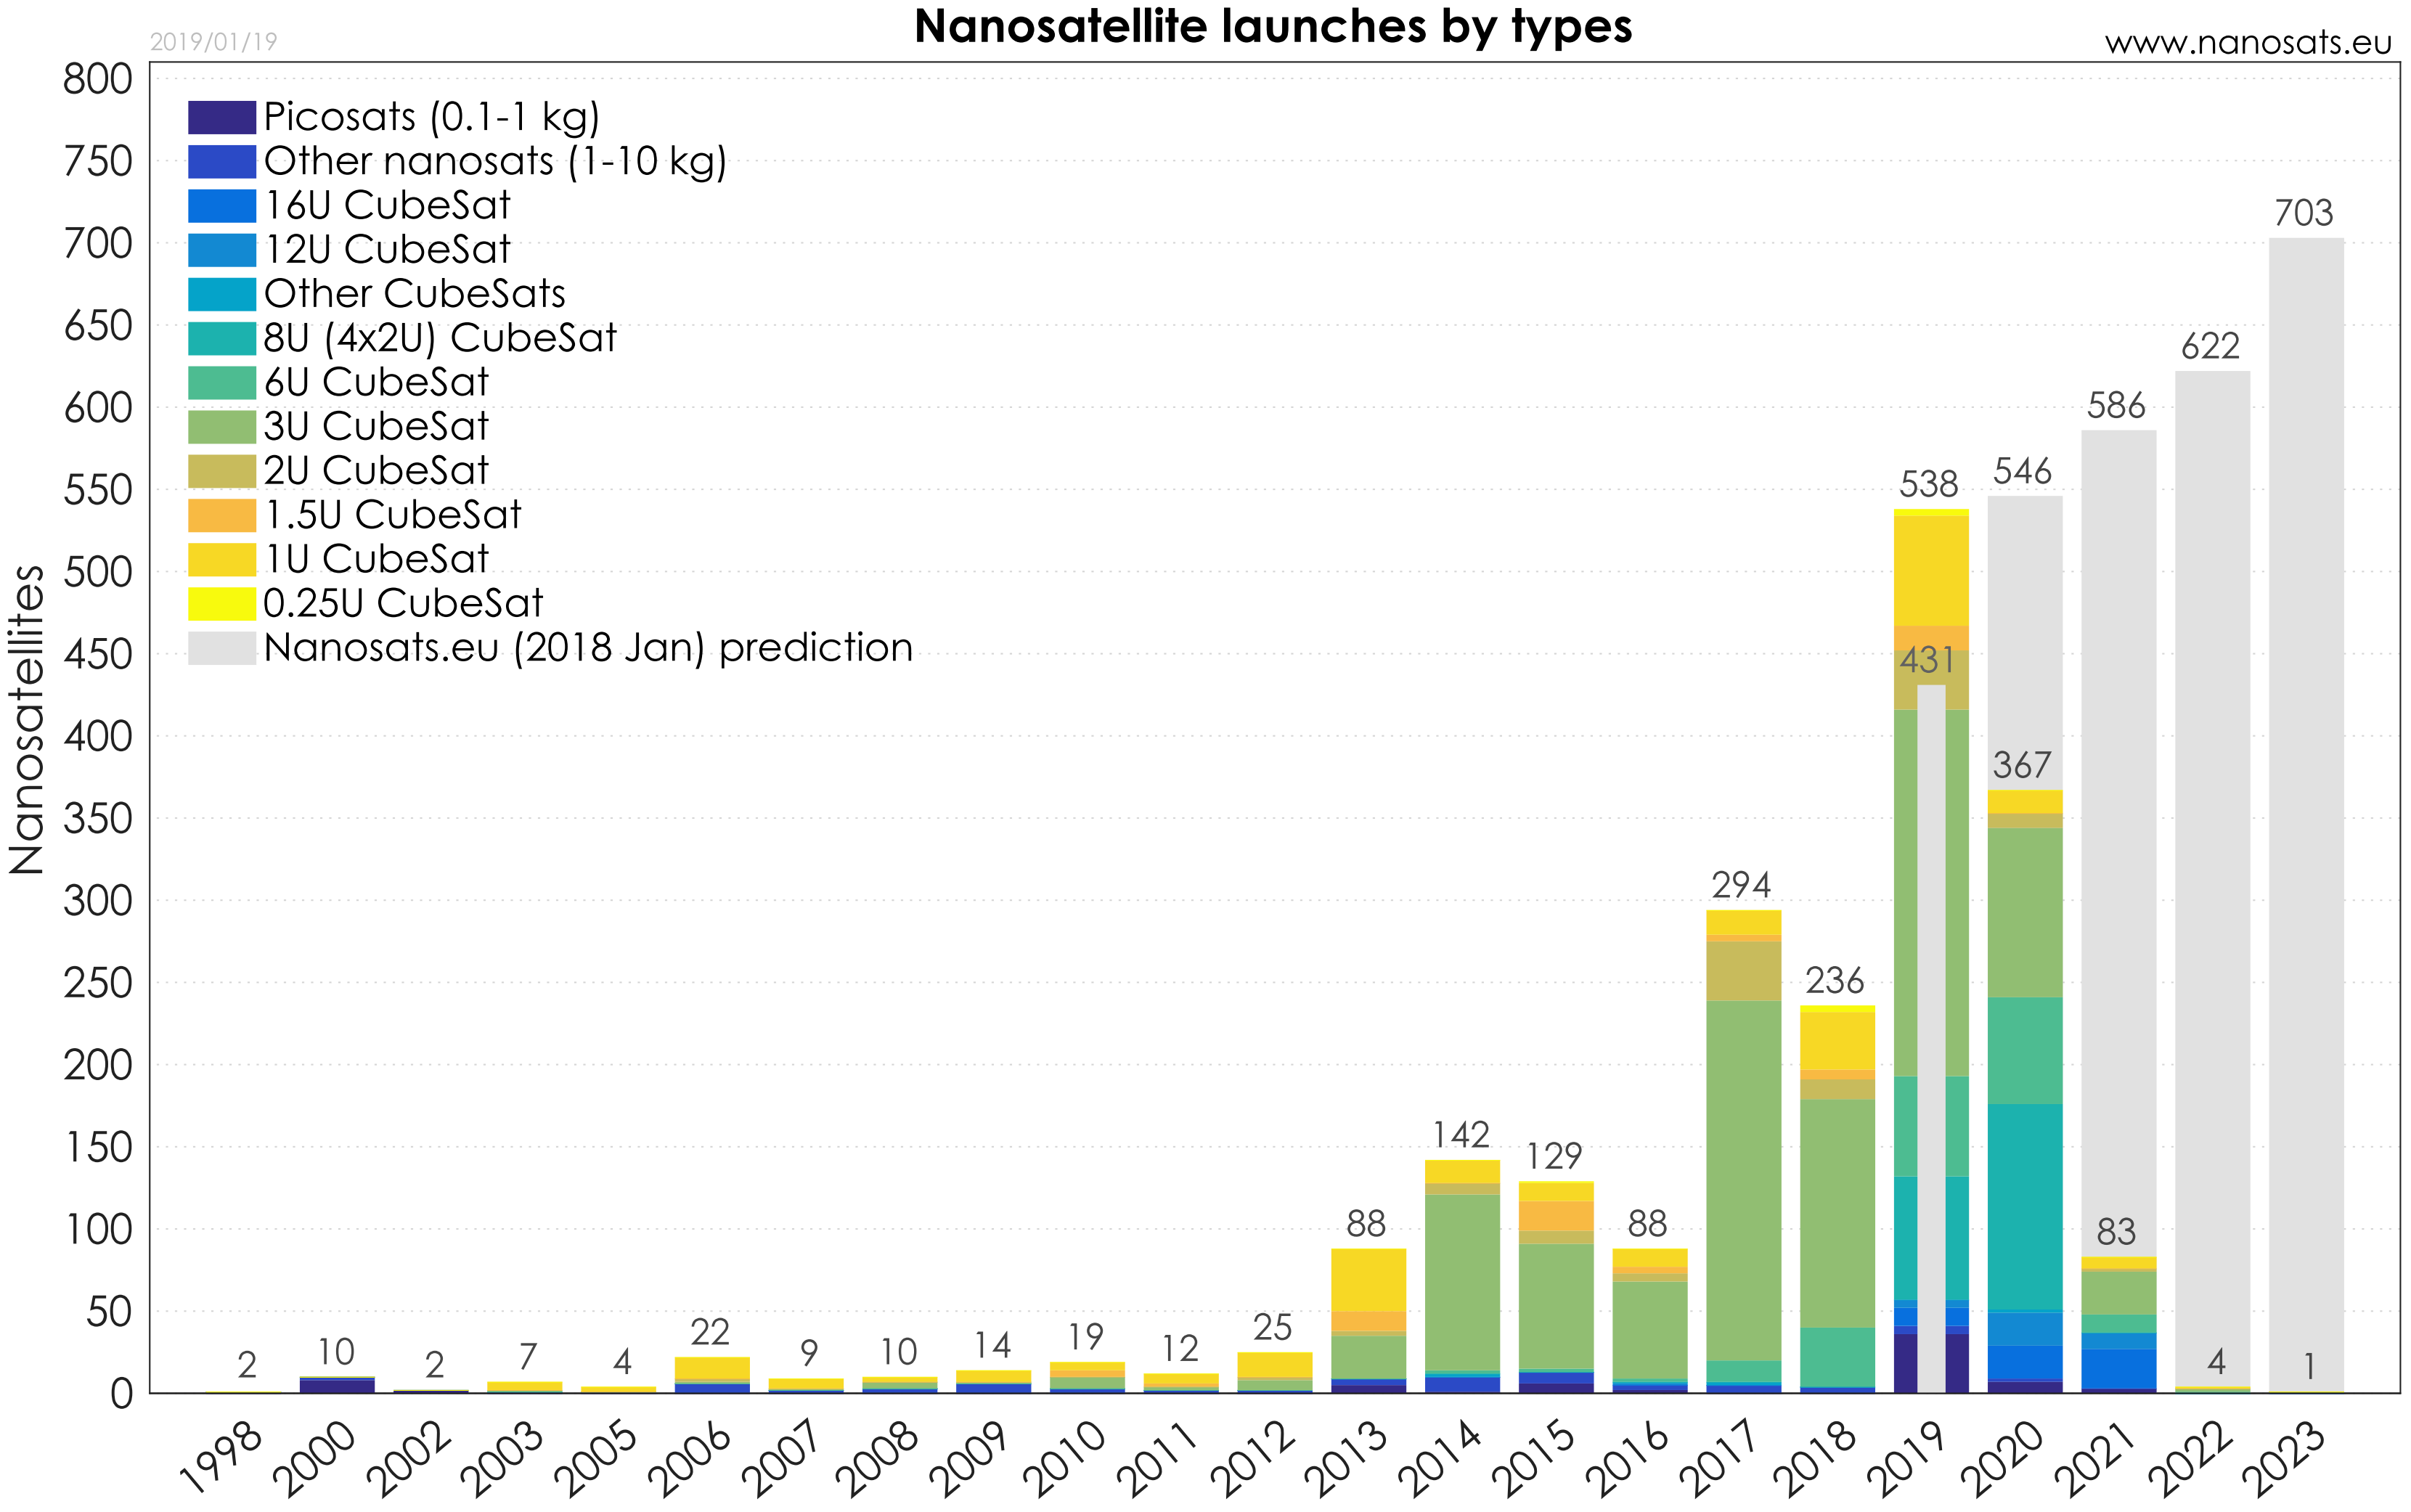
\includegraphics[width=0.80\textwidth]{Nanosats_years_types_2019-01-19_01}
				\caption{Überblick über Nanosatelliten Missionen von 1998 bis 2023}
				\label{fig:NanosatsTypes}
			\end{figure}

	\newpage
	\subsection{Gestaltungsrichtlinien}
Für die Gestaltung von CubeSats gelten eine Reihe von Richtlinien. Als kleinste Einheit (1U) wird ein Würfel mit einer Kantenlänge von 10cm und einer zulässigen Masse von maximal 1,33 kg vorgegeben. Für größere Volumen und Massen können mehrere Einheiten von CubeSats verbunden werden. Satelliten mit 1U, 1.5U, 2U, oder 3U können von dem einheitlichen Startmechanismus (P-Pod) in die Erdumlaufbahn ausgelassen werden. Die Kosten von CubeSat Missionen können gering gehalten werden, indem diese als sekundäre Nutzlast bei Raketenstarts mitfliegen. Für größere Satelliten (6U, 12U, 27U) werden andere Startmechanismen benötigt. Die zugelassene Masse wird auf 2 kg/U angehoben. Weitere Vorschriften gelten für die Folgenden Kriterien:
		\begin{itemize}
			\item \textit{Materialien:} 	\\ Alle bei der Konstruktion verwendeten Materialien müssen den Richtlinien der Air Force Space Command Manual \textbf{[AFSPCMAN 91-710 Volume 3]} entsprechen. Außerdem darf der Masseverlust des Satelliten maximal 1\% betragen.
			\item \textit{Energiespeicher:} \\ Der chemische Energiespeicher darf eine Größe von 100 Wh nicht überschreiten. 
			\item \textit{Aktivierungszeitpunkt:} \\ Während der CubeSat im P-POD verstaut ist müssen alle Systeme ausgeschaltet bleiben. Beim Verlassen der Trägerrakete wird der Satellit aktiviert. Erst 30 Minuten später dürfen Bauteile (z.B. Solarpanele, Antennen, etc...) ausgefahren werden. Bevor die ersten Signale generiert oder gesendet werden müssen mindestens 45 Minuten vergangen sein. 
		\end{itemize}
%Allgemein gelten noch weitere Vorschriften für die verwendeten  Materialien, Kommunikationsfähigkeit, gespeicherte Energie und Aktivierungszeitpunkt der Systeme nach Einsatz in die Umlaufbahn. 
Falls ein Entwurf nicht den Vorschriften entspricht, kann bei dem Betreiber der Trägerrakete eine Sondergenehmigung angefragt werden. Nach einer Reihe von Tests entscheidet dieser ob er die Abweichungen akzeptiert, Änderungen vorgenommen werden müssen, oder ein anderer Anbieter gefunden werden muss. 

	\section{Cubesat Subsysteme}
	%hier Hauptsächlich das Fazit von max kompakt darstellen und refernzieren
		\subsection{Antrieb}
Eines der wichtigsten Subsysteme für Active Debris Removal (ADR) Missionen mit einem CubeSat ist der Antrieb. Er wird für Lageregelung und das Deorbiting des Zielobjekts benötigt.
Für CubeSats stehen nur wenige ausgereifte und erprobte Triebwerke zur Verfügung [Literatur].  Die Miniaturisierung bestehender Technologien stellt eine große Herausforderung dar. Ein hoher TRL ist für die Auswahl besonders Entscheidend, da nur bereits erprobte Technologien für diese Mission genutzt werden sollten.
Im Wesentlichen lassen sich die Antriebsarten in chemische und elektrische Antriebe unterteilen.  Chemische Antriebe generieren im Allgemeinen einen höheren Schub und werden für impulsive Manöver verwendet. Für den Betrieb muss ein großer Gewichtsanteil an Treibstoff einkalkuliert werden. Der spezifische Impuls ist jedoch deutlich niedriger als bei elektrischen Antrieben. Diese bieten auch ein besseres Schub-Leistungs-Verhältnis. Elektrische Antriebe sind jedoch auf eine ausreichende externe Energiequelle angewiesen. Diese wird zwangsläufig benötigt, um die getankte Masse zu beschleunigen [Literatur].
Für genaue Untersuchung und den Vergleich der verschiedenen Triebwerkstypen wird auf [Literatur] verwiesen. Miniaturisierte Versionen von erprobten Triebwerken werden stetig weiterentwickelt und getestet. Es wurden bereits mehrere Miniaturisierte Triebwerke in CubeSatmissionen erfolgreich eingesetzt. In Zukunft sollte es eine wachsende Auswahl an geeigneten Triebwerken für CubeSatmissionen geben. 
		\subsection{Energie - EPS}
		\subsection{Guidance, navigation and control -GNC ADCS}
		Guidance, Navigation and Control (GNC) Subsysteme sind neben den in Kapitel [...] genannten Systemen unabdingbar für ADR Missionen, da diese die Positionsbestimmung als auch die Lagebestimmung und Regelung beinhaltet. Dieses System kann in zwei Hauptbereiche unterteilt werden: der Lage- und Positionsbestimmung, sowie der Lageregelung.
Bei der Lage und Positionsbestimmung kann auf verschiedene Sensoren zurückgegriffen werden. Die absolute Positionsbestimmung erfolgt über eine Bodenstation, welche auch zur Kommunikation mit dem Satelliten verwendet wird. Bei dieser Art der Positionsbestimmung ist es notwendig zu wissen, welchen geplante Erdumlaufbahn der Satellit hat. Diese Methode bezieht sich auf der Zeitdifferenz zwischen Sende- und Empfangszeitpunkt. Deswegen ist die Positionsbestimmung via Bodenradar nicht sehr genau[quelle]. Seit der erfolgreichen Miniaturisierung  von GPS Empfängern werden auch diese zur Positionsbestimmung verwendet. Dies funktioniert solange die GPS Satelliten die Einsatzhöhe von CubeSats überschreiten. Die Lagebestimmung über Startracker erfolgt in dem ein Bild des Himmels mit einem Katalog abgeglichen wird.. Dadurch kann die Lage bei bekannter Position bestimmt werden. Weitere Möglichkeiten sind Sonnen-, Erd- Magnetfeldsensoren, sowie Kreiselinsturmente. Bei Kreiseln wird die Verdrehung im Vergleich zu einem aufgeprägten Inertialsystem gemessen, wodurch die Lage genau bestimmt werden kann. 
Die Regelung  der Lage kann über unterschiedliche Methoden erfolgen. Die einfachste ist eine Drehbewegung um eine der Hauptachsen. Dies führt zu einer Stabilisierung des Satelliten, ist jedoch für eine CubeSat, dessen Aufgabe das Docking und deorbiting beinhaltet, nicht sinnvoll. Dementsprechend kann eine 3 achs-Stabilisierung durchgeführt werden, welche durch Triebwerke und Reaktionsräder durchgeführt werden kann. Diese Art der Lageregelung benötigt ein Reaction Control System (RCS) um unkontrollierte bewegungen zu vermeiden. Die Regelung mittels RCS-Triebwerken geschieht indem Schubimpulse in die jeweilige Richtung gegeben werden. An allen drei Hauptachsen sind Schwungräder montiert. Durch den Antrieb der Räder wird ein Moment erzeugt welches den Satelliten in die gewünschte Lage bringt. Da ein 3-achs System nicht nur Stabilisiert, sondern auch die gewünschte Lage herbeiführen kann, ist dieses System für den viele Fälle optimal.

		\subsection{Command and data handling}
		Das Command- und Data-handling Subsystem (CDHS) ist die Prozessoreinheit, die sich um alles kümmert was mit Software gesteuert wird. Hier werden Daten zu allen Subsystemen und Nutzlasten gesammelt. Das CDHS stellt die Daten bereit, die übertragen werden sollen und führt Befehle aus, die an das Kommunikations Subsystem gesendet werden. 
Es sorgt für die korrekte Einstellung der Solarzellen und Ladung der Batterien. Alle Berechnungen zur Position in der Erdumlaufbahn und der aktuellen Zeit finden hier statt.
Neben dem aktiven Ausführen von Befehlen beobachtet und löst der Prozessor eine Reihe an Problemen, die während der Mission auftreten können.
Die Bestandteile des CDHS sind der Raumflugrechner, die Flugsoftware und ein Speichermedium.

		\subsection{Kommunikation}
		Das Kommunikations Subsystem sorgt bestenfalls für eine dauerhafte Verbindung zur Bodenstation. Aufgezeichnete Daten und eingehende Befehle werden hier von, und an den Cubesat übertragen. Das Subsystem besteht aus den Telemetrie- und Befehlsystemen.
Das Telemetriesystem besteht aus einem oder mehreren Transmittern, welche die vom Prozessor kommenden Daten als Signal an die Bodenstation über die Antennen an Bord des Cubesats aussenden. Die Signale werden als Mikrowelle übertragen und empfangen. Je nach verwendetem System handelt es sich dabei um S-Band-, oder X-Band Wellen. Wellen im X-Band Spektrum können zwar, aufgrund der höheren Frequenz, höhere Bandbreiten erreichen, aber die Technologie ist noch nicht so etabliert wie S-Band Transmitter.
		\subsection{Thermik}
		Die Wärme wird im Vakuum durch Strahlungen und Wärmeleitungen übertragen. Das Wärmemanagement regelt den Bereich der zulässigen Temperaturen für die Sicherstellung einer optimalen Funktionalität und das Überleben des Satelliten. Durch die Massen-, Volumen- und Leistungsbeschränkungen bei miniaturisierten Satelliten, wie dem CubeSat, liegt der Fokus auf den passiven Wärmereglungstechnologien, da die Fortschritte bei der Entwicklung von miniaturisierten aktiven Wärmeregelungsmethoden begrenzt ist. Passive Technologien sind mit geringen Kosten, Volumen, Gewicht und Risiko verbunden und erfordern keine interne Eingangsleistung für die Wärmeregulierung. Thermische Beschichtungen, Wärmerohre, Sonnenschirme, Wärmebänder und Multi-Layer Insulation (MLI) sind passive Methoden für die Regulierung des thermischen Gleichgewichtes. Die aktiven Methoden, wie elektrische Widerstandsheizungen, Kühler oder kryogene Materialien, sind mit höherer Präzision und interner Eigenleistung verbunden. Die Verwendung von aktiven Systemen ist bei temperaturempfindlichen Geräten und nicht ausreichender, passiver Systeme für eine Aufrechterhaltung der Betriebstemperatur vielversprechender [Literatur NASA Sota].

		\subsection{Struktur}
		Die Strukturen werden in Primär- und Sekundärestrukturen unterteilt. Die Primärstruktur ist thermischen und dynamischen Beeinflussungen ausgesetzt, denen sie entgegenwirken muss. Des Weiteren sorgt es für Lastübertragung während des Starts und des Einsatzes. Elektromagnetische Strahlungen, Drücke und innere Wärmeleitungen sind weitere Faktoren die einen großen Einfluss auf das Gehäuse haben und deshalb mit einbezogen werden müssen. Die Begrenzungen bei der Oberfläche und bei dem Volumen sorgen für Einschränkungen. Infolgedessen sollte sie effizient ausgelegt werden. Komponenten die nur sich selbst tragen müssen, wie Sonnenkollektoren, zählen zu den Sekundärstrukturen auf die nicht näher eingegangen wird, da sie bei einem Ausfall die Integrität des Raumfahrzeugs nicht beeinträchtigt. Die Primärstrukturen werden als COTS-Strukturen und kundenspezifisch bearbeitet oder gedruckte Komponenten auf dem Markt angeboten. Generell besteht das Gehäuse aus metallischen und nichtmetallischen Materialien und wird von der Betriebsumgebung des Satelliten bestimmt [Literatur: NASA Sota].
				
	\section{RDVDO Mechanismen} das kann ausführlich sein
		\subsection{Docking Strategien}
						\textbf{Roboterarm}
						\textbf{Fangnetz}
						\textbf{Adhäsiv Docken}
						%Übersichtstabelle/Graphik: sihe die Quellen die ich am 15.05.2019 gezeigt habe
		\newpage
		\subsection{Bionische Materialien}
		Gecko-inspirierte mikrostrukturierte Oberflächen scheinen eine vielversprechende Lösung für das Dockingproblem bei ADR Missionen zu sein. Mittels trockener Adhäsion können Geckos in der Natur an Oberflächen haften. Durch die hierarchische Struktur ihrer Füße entstehen Van-der-Waals-Wechselwirkungen. Die kleinsten Fasern haben einen Durchmesser und eine Länge von einigen Nanometern. Insgesamt besitzt ein Gecko über 500000 Hafthaare an einem Fuß. Sie bilden eine Flexible Struktur, die problemlos an glatten oder rauen Oberflächen haftet. Da für das Docking etwas genutzt werden muss, das den Bedingungen im Weltraum wie Vakuum, Strahlung und Kälte standhält, sollen Geckomaterialien für diese Anwendung näher untersucht werden. Besonders vorteilhaft ist das zerstörungsfreie Andocken mittels der Geckostruktur, was das Risiko neu entstehender Trümmerteile verringert.
		Van-der-Waals-Wechselwirkungen sind grundlegend molekulare Wechselwirkungen. Indem temporäre Umverteilungen von Elektronen in einem Molekül stattfinden entstehen Bereiche die unterschiedlich geladen sind (Dipole). Diese haben Auswirkungen auf benachbarte Moleküle. Es entsteht eine Kettenreaktion von Dipolbildungen, die zu Anziehungskräften zwischen Positiv und Negativ geladenen Bereichen naher Moleküle führt. Jedes Kleinsthaar baut dabei eine Haftkraft auf. Mit einer steigenden Anzahl an Bindungsstellen erhöht sich auch die gesamte Haftkraft. Außerdem wird die Ablösekraft größer, desto kleiner die Strukturdurchmesser sind, da auf einer kleinen Fläche eine Vielzahl an Kontakten entstehen[Literatur].
	Mit dem heutigen Stand der Technik ist es möglich diese Mikrostrukturen kostengünstig und schnell mit bestimmten Verfahren reproduzierbar herzustellen. Diese synthetisch hergestellten Mikrostrukturen erreichen bereits ähnliche Haftkräfte wie ihre natürlichen Vorbilder. Mit den Strukturen aus \abb{fig:Gecko1} wurden Haftkräfte von 10 $\frac{N}{mm^{2}}$ und Scherbeanspruchungen (Ablösekräfte)  von 2 $\frac{N}{mm^{2}}$ gemessen.
	\begin{figure}[h]
	\centering
		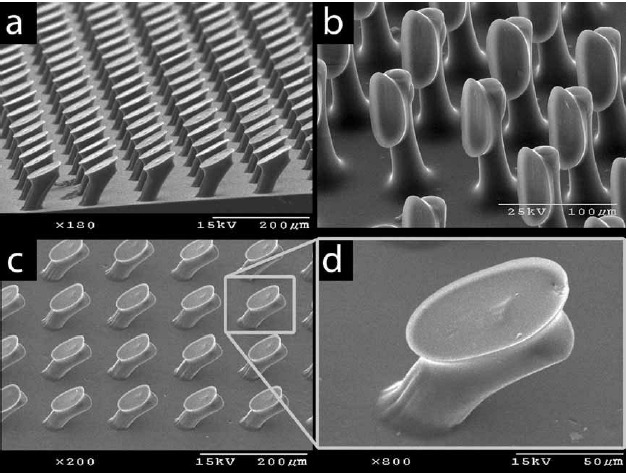
\includegraphics[width=0.70\textwidth]{Gecko1}
	\caption{Aufnahme einer Mikrostruktur mit 35 um Durchmesser. Strukturen weisen unterschiedliche Winkel auf: a) 	34\textdegree{}  b) 90\textdegree{}  c),d) 23\textdegree{} [Literatur]}
	\label{fig:Gecko1}
\end{figure}
	Eine genaue Auflistung der erreichten Haftkräfte für die verschiedenen Ausführungen der Mikrostruktur und Belastungsfälle ist in [Literatur Tab 1] zu finden.
Polydimethylsiloxan (PDMS) Strukturen erreichen maximale Scherkräfte in Haftrichtung von 34,8 $\frac{N}{mm^{2}}$ und einer Normalkraft von 10,8 $\frac{N}{mm^{2}}$.
PDMS Strukturen wurden bereits erfolgreich in der Schwerelosigkeit getestet. Diese konnten an einem Greifer verschiedene Objekte einfangen und bewegen [Literatur].

Außerdem wurde durch mehrere Versuchsreihen nachgewiesen, dass Temperatur und Vakuum kaum einen Einfluss auf die Leistungsdaten haben. Verschiedene Mikrostrukturen wurden einer thermischen Wechselbeanspruchung zwischen 125 und  -125 \textdegree{} C unterzogen und daraufhin in Vakuum und Normalbedingungen getestet. Durch die Temperatur ist kein Einfluss zu verzeichnen. Das Vakuum ruft nur vernachlässigbare Änderungen in Vorspannung und Haftung hervor   [Literatur Fig.11]. Durch Tests mit verschiedenen Materialien konnte festgestellt werden, dass die Oberfläche, an der die Struktur haften soll einen relativ geringen Einfluss auf die Haftung hat [Literatur Fig.16]. 

Bei der technischen Anwendung ist zu beachten, dass es eine Haftrichtung und eine Ablöserichtung in der Struktur gibt. Die haltbaren Scherkräfte in Ablöserichtung sind somit um bis zu Faktor 10 geringer als in Haftrichtung.
\begin{figure}[h]
	\centering
		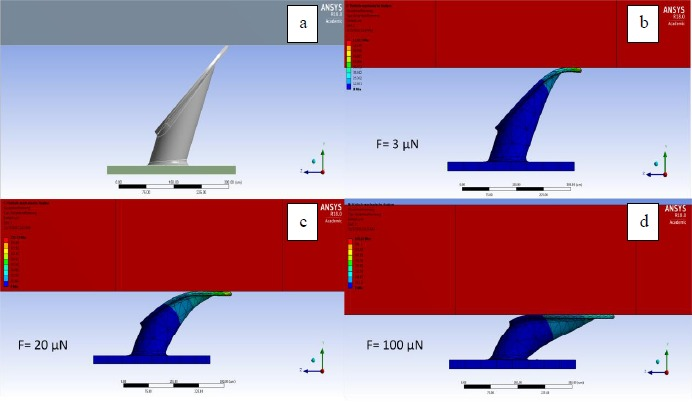
\includegraphics[width=0.70\textwidth]{Gecko2}
	\caption{Simulation des Verformungsverhaltens der Mikrostruktur bei Haftberührung [Literatur]}
	\label{fig:Gecko2}
\end{figure}	
	In der Simulation (\abb{fig:Gecko2}) ist gut zu erkennen, dass die Mikrosäulen mit dem Haftprofil in eine vorbestimmte Richtung belastet werden sollen. Andernfalls können sie nicht die maximale Haftfläche nutzen und es geht Haftkraft verloren [Literatur, Abb.26 u. ff]. 
Allgemein wurde festgestellt, dass die Normalkraft und Scherkräfte mit Erhöhung der Anpresskraft steigen. Optimaler Halt sollte also mit einer Anpresskraft erreicht werden [Literatur]. Zukünftig besteht die Möglichkeit verschiedene Formen der Hafthaare zu kombinieren, um deren Vorteile zu nutzen. 

Es existiert bereits ein Andockmechanismus ( \abb{fig:Gecko3})  mit nach  European Cooperation for Space Standardization (ECSS) Standards getesteter Gecko Mikrostruktur. Um die Funktionsgrenzen des Mechanismus zu bestimmen,  sollen in naher Zukunft Dockingmanöver im ELISSA-Labor simuliert werden [Literatur].

\begin{figure}[htbp]
	\centering
		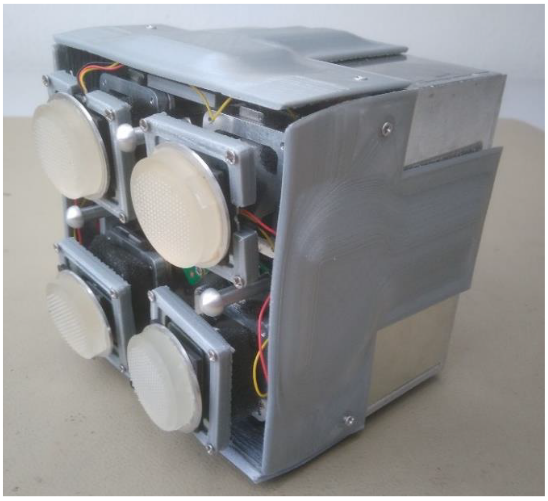
\includegraphics{graphics/Gecko3.PNG}
	\caption{Gecko Dockingmechanismus}
	\label{fig:Gecko3}
\end{figure}


		
						%\textbf{Was sind Geckomaterialen}
						%\textbf{Bisher getestete Gecko-Materialien}
						%\textbf{Bisherige Erfolge}
						%\textbf{State of the Art}
						%\textbf{Problematik}